\chapter{Services}

{Help Developer to built better apps and don't focus on operation . Save crucial development time and ship a high-quality, bug-free app.
	There are three main categories of services in Firebase, we will discus there services in details .
	}
\begin{figure}[H]
	\centering
	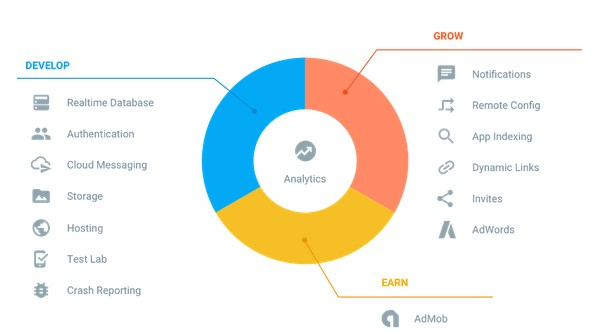
\includegraphics[height=3in]{./TeX_files/Pic1}
	\caption[optional caption]{Firebase Services}
	\label{Fig:Tobias}
\end{figure}
%Figure \ref{Fig:Tobias} Shows Tobias in Tree

\section{Analytics}
\subsection{Firebase Analytics}
\subitem{
	At the heart of Firebase is Firebase Analytics, a free App measurement solution and unlimited analytics solution. See user behavior and measure attribution from a single dashboard. 
	}
\section{Develop}
\subsection{Firebase Cloud Messaging}
\subitem{
	Firebase Cloud Messaging (FCM) s a cross-platform solution for messages and notifications for Android, iOS, and web applications. Deliver and receive messages reliably.
	Using FCM, you can notify a client app that new email or other data is available to sync. You can send notification messages to drive user and retention. a message can transfer a payload of up to 4KB to a client app.
	}
\subsection{Auth}
\subitem{
	this most important thing for most apps need to know the identity of a user.Knowing a user's identity allows an app to save user data in the cloud.It supports authentication using passwords, popular identity providers like Google, Facebook and Twitter, and more.
	}
\subsection{Realtime database}
\subitem{
	Store and sync data with our NoSQL cloud database. Data is synced across all clients in realtime, and remains available when your app goes offline.Data is stored as JSON and synchronized in realtime to every connected client.
	}
\subsection{Storage}
\subitem{
	
	Cloud Storage is built for app developers who need to store and serve user-generated content, such as photos or videos.The Firebase SDKs for Cloud Storage add Google security to file uploads and downloads for your Firebase apps
	}
\subsection{Hosting}
\subitem{
	Firebase Hosting serve your web App,provides fast and secure static hosting for your web app.production-grade web content hosting for developers. With Hosting, you can quickly and easily deploy web apps and static content
	}
\subsection{Test Lab for Android}
\subitem{
	Firebase Test Lab for Android provides cloud-based infrastructure for testing Android apps. With one operation, you can testing your app across a wide variety of devices. Test results—including logs, videos, and screenshots—are made available in your project in the Firebase console. Test Lab can exercise your app automatically, looking for crashes.
	}
\subsection{Crash Reporting}
\subitem{
	Crash Reporting create reports of the error in Apps, Errors are grouped into issues based on having similar stack, and and notify in your project in the firebase console. 
	}
\section{Grow}
\subsection{Notifications}
\subitem{
	Firebase Notifications is a free service that enables targeted user notifications for mobile app developers. Firebase Notifications provides an option for developers a flexible notification platform that requires minimal coding effort to get started, and a graphical console for sending messages. Using the Notifications console GUI.
	}
\subsection{Remote Config}
\subitem{
	
	Remote Config change the behavior and appearance of your app without publishing an app update.it a cloud service that lets you change the behavior and appearance of your app without requiring users to download an app update. When using Remote Config, you create in-app default values that control the behavior and appearance of your app. Then, you can later use the Firebase console to override in-app default values for all app users. Your app controls when updates are applied, and it can frequently check for updates and apply them .
	}
\subsection{App Indexing}
\subitem{
	Firebase App Indexing gets your app into Google Search. If users have your app installed, they can launch your app and go directly to the content they're searching for. 
	}
\subsection{Dynamic Links}
\subitem{
	 Firebase Dynamic Links are links that work the way you want, on multiple platforms.With Dynamic Links, your users get the best available experience for the platform they open your link on. If a user opens a Dynamic Link on iOS or Android, they can be taken directly to the linked content in your native app. If a user opens the same Dynamic Link in a desktop browser, they can be taken to the equivalent content on your website.
	}
\subsection{Invites}
\subitem{
	Firebase Invites are an out-of-the-box solution for app  sharing via email or SMS. To customize the invitation user experience, or to generate links programmatically
	}
\subsection{Google AdWords}
\subitem{
	Reach potential customers with online ads.
}